% Project report, MATH F428. Build: cd report && tectonic report.tex  (numbers and figures come from ../slides/beamer after make_figures.py)
\documentclass[11pt,a4paper]{article}
\usepackage[margin=2.3cm]{geometry}
\usepackage{graphicx,booktabs,amsmath,amssymb,hyperref,float,caption,xcolor}
\hypersetup{colorlinks=true,urlcolor=blue!60!black,linkcolor=blue!60!black}
\graphicspath{{../slides/beamer/fig/}{../figures/}}
\newcommand{\pmtwo}{PM$_{2.5}$}
\newcommand{\ugm}{$\mu$g/m$^3$}
\newcommand{\ugmm}{\ensuremath{\mu\mathrm{g/m^3}}}
\newcommand{\nDays}{2{,}009}
\newcommand{\nWeeks}{287}
\newcommand{\nWeeksModel}{261}
\newcommand{\nTrain}{209}
\newcommand{\pctPoor}{54}
\newcommand{\pmMean}{121}
\newcommand{\winterMean}{217}
\newcommand{\monsoonMean}{48}
\newcommand{\ratioWM}{4.5}
\newcommand{\skewRaw}{1.66}
\newcommand{\skewLog}{\ensuremath{-}0.14}
\newcommand{\corrRaw}{0.94}
\newcommand{\corrLog}{\ensuremath{-}0.09}
\newcommand{\sdRatioRaw}{7.9}
\newcommand{\sdRatioLog}{1.5}
\newcommand{\Fs}{0.90}
\newcommand{\Ft}{0.18}
\newcommand{\seasRatio}{17}
\newcommand{\declAll}{22}
\newcommand{\acfOne}{0.87}
\newcommand{\acfHalf}{\ensuremath{-}0.43}
\newcommand{\acfYear}{0.68}
\newcommand{\acfDOne}{0.29}
\newcommand{\adfPLog}{\ensuremath{4.8\times10^{-4}}}
\newcommand{\kpssLog}{0.058}
\newcommand{\adfPDiff}{\ensuremath{1.7\times10^{-4}}}
\newcommand{\kpssDiff}{0.341}
\newcommand{\stnFirst}{10}
\newcommand{\stnSecond}{8}
\newcommand{\stnLast}{37}
\newcommand{\varLagAic}{4}
\newcommand{\varLagBic}{2}
\newcommand{\portP}{0.17}
\newcommand{\spearWind}{\ensuremath{-}0.22}
\newcommand{\spearRh}{\ensuremath{-}0.26}
\newcommand{\gWindP}{\ensuremath{<10^{-12}}}
\newcommand{\gRhP}{\ensuremath{1.2\times10^{-11}}}
\newcommand{\gBothP}{\ensuremath{<10^{-12}}}
\newcommand{\gRevWindP}{0.12}
\newcommand{\gRevRhP}{0.62}
\newcommand{\gWindPc}{\ensuremath{<10^{-12}}}
\newcommand{\gRhPc}{\ensuremath{9.7\times10^{-9}}}
\newcommand{\nestRone}{0.123}
\newcommand{\nestRtwo}{0.128}
\newcommand{\nestDR}{0.005}
\newcommand{\nestP}{0.47}
\newcommand{\nestRsame}{0.17}
\newcommand{\sarMA}{\ensuremath{-}0.99}
\newcommand{\sarMASE}{8}
\newcommand{\lbAll}{\ensuremath{<10^{-12}}}
\newcommand{\lbTen}{0.49}
\newcommand{\lbTwentySix}{0.10}
\newcommand{\lbFiftyTwo}{0.016}
\newcommand{\maeNaiveSeventeen}{38.4}
\newcommand{\maeNaiveEighteen}{29.0}
\newcommand{\maeNaiveNineteen}{30.3}
\newcommand{\maeNaiveAvg}{29.6}
\newcommand{\rmseNaiveAvg}{43.1}
\newcommand{\mapeNaiveAvg}{30}
\newcommand{\meNaiveAvg}{\ensuremath{-}8.1}
\newcommand{\covNaiveSeventeen}{88}
\newcommand{\covNaiveEighteen}{94}
\newcommand{\covNaiveNineteen}{92}
\newcommand{\maeMeanSeventeen}{31.0}
\newcommand{\maeMeanEighteen}{21.8}
\newcommand{\maeMeanNineteen}{27.8}
\newcommand{\maeMeanAvg}{24.8}
\newcommand{\rmseMeanAvg}{34.7}
\newcommand{\mapeMeanAvg}{27}
\newcommand{\meMeanAvg}{\ensuremath{-}10.8}
\newcommand{\covMeanSeventeen}{62}
\newcommand{\covMeanEighteen}{92}
\newcommand{\covMeanNineteen}{81}
\newcommand{\maeHWSeventeen}{44.7}
\newcommand{\maeHWEighteen}{19.2}
\newcommand{\maeHWNineteen}{32.2}
\newcommand{\maeHWAvg}{25.7}
\newcommand{\rmseHWAvg}{36.1}
\newcommand{\mapeHWAvg}{30}
\newcommand{\meHWAvg}{\ensuremath{-}14.7}
\newcommand{\covHWSeventeen}{64}
\newcommand{\covHWEighteen}{94}
\newcommand{\covHWNineteen}{86}
\newcommand{\maeSarimaSeventeen}{72.3}
\newcommand{\maeSarimaEighteen}{21.1}
\newcommand{\maeSarimaNineteen}{27.5}
\newcommand{\maeSarimaAvg}{24.3}
\newcommand{\rmseSarimaAvg}{34.5}
\newcommand{\mapeSarimaAvg}{27}
\newcommand{\meSarimaAvg}{\ensuremath{-}11.7}
\newcommand{\covSarimaSeventeen}{23}
\newcommand{\covSarimaEighteen}{94}
\newcommand{\covSarimaNineteen}{85}
\newcommand{\maeHarmSeventeen}{29.4}
\newcommand{\maeHarmEighteen}{22.5}
\newcommand{\maeHarmNineteen}{26.4}
\newcommand{\maeHarmAvg}{24.5}
\newcommand{\rmseHarmAvg}{34.0}
\newcommand{\mapeHarmAvg}{26}
\newcommand{\meHarmAvg}{\ensuremath{-}10.7}
\newcommand{\covHarmSeventeen}{65}
\newcommand{\covHarmEighteen}{92}
\newcommand{\covHarmNineteen}{86}
\newcommand{\maeCombSeventeen}{38.2}
\newcommand{\maeCombEighteen}{20.1}
\newcommand{\maeCombNineteen}{27.6}
\newcommand{\maeCombAvg}{23.8}
\newcommand{\rmseCombAvg}{33.7}
\newcommand{\mapeCombAvg}{27}
\newcommand{\meCombAvg}{\ensuremath{-}11.8}
\newcommand{\dmPNaive}{0.03}
\newcommand{\dmDNaive}{4.8}
\newcommand{\dmPHW}{0.57}
\newcommand{\dmDHW}{0.9}
\newcommand{\dmPSarima}{0.49}
\newcommand{\dmDSarima}{\ensuremath{-}0.5}
\newcommand{\dmPHarm}{0.74}
\newcommand{\dmDHarm}{\ensuremath{-}0.3}
\newcommand{\dmPComb}{0.08}
\newcommand{\dmDComb}{\ensuremath{-}0.9}
\newcommand{\covMinSeventeen}{23}
\newcommand{\covMaxSeventeen}{88}
\newcommand{\covMinEighteen}{92}
\newcommand{\covMaxEighteen}{94}
\newcommand{\covMinNineteen}{81}
\newcommand{\covMaxNineteen}{92}
\newcommand{\bestAvgModel}{Combination}
\newcommand{\widthNaiveNineteen}{160}
\newcommand{\widthNaiveSeventeen}{167}
\newcommand{\widthMeanNineteen}{103}
\newcommand{\widthMeanSeventeen}{77}
\newcommand{\widthHWNineteen}{173}
\newcommand{\widthHWSeventeen}{131}
\newcommand{\widthSarimaNineteen}{133}
\newcommand{\widthSarimaSeventeen}{36}
\newcommand{\widthHarmNineteen}{112}
\newcommand{\widthHarmSeventeen}{90}
\newcommand{\hwGamma}{\ensuremath{7.3\times10^{-5}}}
\newcommand{\hwAlpha}{0.27}
\newcommand{\onePers}{30.7}
\newcommand{\oneMean}{24.8}
\newcommand{\oneNo}{21.5}
\newcommand{\oneLag}{22.1}
\newcommand{\oneOracle}{20.0}
\newcommand{\oneLagPct}{2.6}
\newcommand{\oneOraclePct}{\ensuremath{-}7.2}
\newcommand{\oneLagP}{0.04}
\newcommand{\oneOracleP}{0.08}
\newcommand{\lockActual}{49}
\newcommand{\lockFcHarm}{95}
\newcommand{\lockFcMean}{97}
\newcommand{\lockGapHarm}{\ensuremath{-}49}
\newcommand{\lockGapMean}{\ensuremath{-}50}
\newcommand{\lockGapMin}{\ensuremath{-}44}
\newcommand{\lockGapMax}{\ensuremath{-}50}
\newcommand{\lockPreHarm}{\ensuremath{-}16}
\newcommand{\lockAdjMin}{\ensuremath{-}34}
\newcommand{\lockAdjMax}{\ensuremath{-}41}
\newcommand{\lockAdjHarm}{\ensuremath{-}39}
\newcommand{\lockPlaceboHarm}{\ensuremath{-}14}
\newcommand{\janMaeMin}{28}
\newcommand{\janMaeMax}{42}
\newcommand{\preBiasLo}{7}
\newcommand{\preBiasHi}{17}
\newcommand{\preBiasMin}{\ensuremath{-}7}
\newcommand{\preBiasMax}{\ensuremath{-}17}
\newcommand{\janMaeHarm}{35.7}
\newcommand{\janMaeMean}{36.4}
\newcommand{\lockUsualLo}{\ensuremath{-}31}
\newcommand{\lockUsualHi}{23}
\newcommand{\lockWinMinHarm}{\ensuremath{-}36}
\newcommand{\lockWinMin}{\ensuremath{-}52}
\newcommand{\lockWinMax}{42}
\newcommand{\exWeek}{3}
\newcommand{\exYa}{188}
\newcommand{\exYb}{272}
\newcommand{\exYc}{238}
\newcommand{\exYd}{197}
\newcommand{\exMean}{221}
\newcommand{\exNaive}{197}
\newcommand{\declWeeks}{26}
\newcommand{\aicA}{73.2}
\newcommand{\aicB}{53.9}
\newcommand{\aicC}{39.4}
\newcommand{\aicD}{45.2}
\newcommand{\aicE}{57.5}
\newcommand{\aicBest}{39.4}
\newcommand{\aicGap}{5.8}
\newcommand{\kHarmLo}{6}
\newcommand{\kHarmHi}{7}
\newcommand{\lockShareHW}{3}
\newcommand{\lockShareAdjHW}{8}
\newcommand{\lockMinHW}{\ensuremath{-}46}
\newcommand{\lockShareSarima}{1}
\newcommand{\lockShareAdjSarima}{5}
\newcommand{\lockMinSarima}{\ensuremath{-}52}
\newcommand{\lockShareHarm}{0}
\newcommand{\lockShareAdjHarm}{0}
\newcommand{\lockMinHarm}{\ensuremath{-}36}
\newcommand{\lockShareMean}{0}
\newcommand{\lockShareAdjMean}{0}
\newcommand{\lockMinMean}{\ensuremath{-}36}

\setlength{\parskip}{4pt}\setlength{\parindent}{0pt}
\renewcommand{\arraystretch}{1.1}
\title{Forecasting Delhi's \pmtwo{}: Seasonality, Weather Predictability and a Rolling-Origin Forecasting Study}
\author{Kushagra Singh \and Yatin JM \and Aryan Choudhary\\ BITS Pilani, Goa \,--\, MATH F428 Time Series Analysis}
\date{November 2026}
\begin{document}
\maketitle
\begin{abstract}
We study daily \pmtwo{} in Delhi from January 2015 to July 2020 (CPCB monitors; ERA5 wind and humidity). \pmtwo{} has a very strong annual cycle (winter \ratioWM$\times$ the monsoon) and a slow downward drift. After removing the cycle, wind and humidity anomalies \emph{predict} \pmtwo{} for about a week (Granger causality in a VAR, robust to lag order, differencing, HAC errors and rain/temperature controls), but their information is gone at the weekly scale: last week's weather adds nothing for this week, and even the same week's weather, unknown in advance, improves a one-week forecast by only \fcOneOracle\%. For 52-week forecasts we compare climatology, Fourier-term regression with ARMA errors, SARIMA, linear regression and a small LSTM on three expanding-window origins. A smooth Fourier+ARMA model matches or slightly beats climatology; SARIMA with seasonal differencing is fragile, and the LSTM is clearly worse. We fix several diagnostic and design errors found in an earlier draft (residual burn-in, missing constant, leakage), calibrate prediction intervals out of sample, and produce a monthly 2020 outlook that correctly flags the lockdown as a \fcLockPct\% fall below the no-lockdown forecast.
\end{abstract}

\section{Introduction}
Delhi's air is Poor or worse (PM$_{2.5}>90$ \ugm{}) on \pctPoor\% of days in our sample, and the pattern repeats every winter. We ask two questions: \textbf{Q1} (explain) does weather predict \pmtwo{}, and over what horizon? \textbf{Q2} (forecast) how well can \pmtwo{} be forecast one week and 52 weeks ahead, and which model should be trusted? The project was reviewed independently three times; every concrete claim of those reviews was re-tested on the data, and the verdicts are in \texttt{docs/REVIEW\_RESPONSES.md} (summarised in Section~\ref{sec:review}). Because the data end in July 2020, the deliverable is a \emph{historical forecasting study} (backtests for 2017--2019 and an outlook for 2020 made in December 2019), not a current health advisory.

\section{Data and cleaning}
\pmtwo{} (and NO$_2$, SO$_2$) are the CPCB city-level daily values for Delhi from the Kaggle dataset \texttt{rohanrao/air-quality-data-in-india}: 2{,}009 days, 1 Jan 2015 to 1 Jul 2020, with 2 missing \pmtwo{} values (interpolated; gaps $\le3$ days are interpolated, longer ones are left missing). Wind speed, relative humidity, temperature and precipitation are ERA5 reanalysis values for central Delhi (28.61$^\circ$N, 77.21$^\circ$E) from the Open-Meteo archive. Forecasting uses weekly means (weeks ending Sunday, 287 weeks). Modelling is on $\log$ \pmtwo{}; a back-transformed forecast $\exp(\mu)$ is a \emph{median}, and mean forecasts use $\exp(\mu_h+\sigma_h^2/2)$ with the horizon-specific $\sigma_h$. The 2020 lockdown never enters model selection.

\section{Exploratory analysis}
\subsection{Seasonality and the log transform}
Winter (Nov--Jan) averages \winterMean{} \ugm{} against \monsoonMean{} in the monsoon (\ratioWM$\times$). An STL decomposition of the weekly log series gives a seasonal strength $F_S=\Fs$ on the training years (0.89 on the full sample). The spread of daily \pmtwo{} grows with its level (monthly mean and SD correlate at 0.95; the largest monthly SD is \sdRatioRaw$\times$ the smallest); after the log it varies only \sdRatioLog$\times$ and the skewness falls from \skewRaw{} to \skewLog{}. The Box-Cox $\lambda$ is \boxcox{} (about 0.10 on the training years), i.e. close to the log. Some volatility clustering remains in the daily series (ARCH-LM \archRaw{} $\to$ \archLog{}); we check it again on the weekly forecast residuals, where it is absent (ARCH-LM(4) $p=0.87$).
\begin{figure}[H]\centering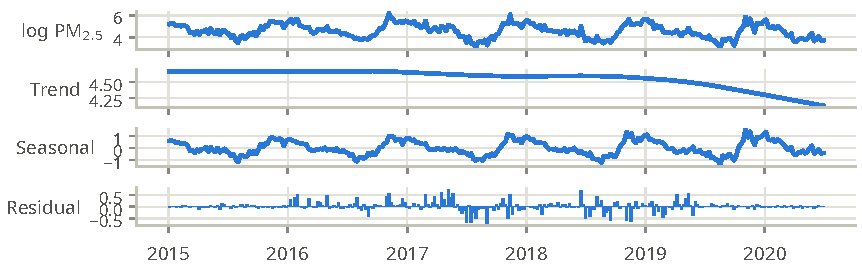
\includegraphics[width=0.95\linewidth]{stl.pdf}\caption{STL decomposition of weekly log \pmtwo{}.}\end{figure}

\subsection{Stationarity and the hidden drift}
ADF and KPSS (opposite null hypotheses) on 2015--2018 weekly log \pmtwo{} are both consistent with stationarity, as is the seasonal difference; a further first difference over-differences (lag-1 autocorrelation $-0.46$). So $d=0$. But KPSS on the \emph{raw level} is dominated by the large seasonal cycle. Removing a day-of-year climatology reveals a slow decline: the KPSS statistic of the anomaly is 0.90 on 2015--18 and 2.0 on 2015--19 (5\% critical value 0.46), and the mean log anomaly falls from $+0.10$ in 2016 to $-0.19$ in 2019. The level is therefore \emph{not} constant, which drives the model design in Section~\ref{sec:fc}.

\subsection{Is the decline real? A station-level check}
The city series is the mean over reporting stations (correlation 0.995 with the station-level mean), and the number of stations reporting \pmtwo{} rose from 10 and 8 (2015, 2016) to 37 (2018, 2019), so a change in the station mix could create a spurious decline. A fixed panel of six long-running stations (at least 60 days in each year) falls by \declPanel\% between 2016 and 2019, all stations by \declAll\%, and the city series after regressing out wind, humidity and temperature by \declWx\%. We conclude that most of the decline is real, while stressing that the panel is small and thin in 2017.
\begin{figure}[H]\centering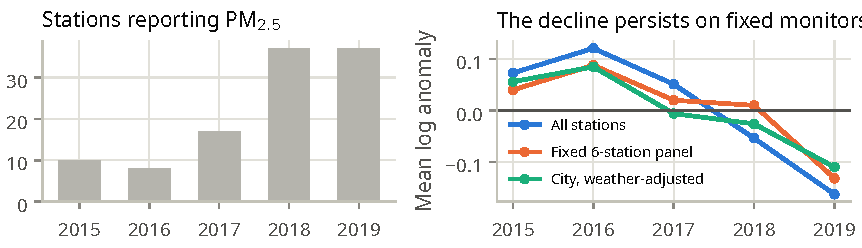
\includegraphics[width=0.85\linewidth]{fc_station.pdf}\caption{Left: stations reporting; right: mean log anomaly by year for all stations, the fixed panel and the weather-adjusted city series.}\end{figure}

\section{Does weather predict \pmtwo{}? (Q1)}
Wind, humidity and log \pmtwo{} are deseasonalised with a smoothed day-of-year climatology (31-day circular window; leap years handled by mapping 29 Feb to day 59) and fitted in a VAR(4) (lag by AIC; BIC picks 2; stable, largest root modulus 0.81; portmanteau $p=0.17$).
\paragraph{Granger causality.} Joint tests that lags 1--$k$ of wind or humidity add nothing to the \pmtwo{} equation are rejected at every $k=1,\dots,7$ ($p<10^{-9}$). With HAC (Newey-West) errors the 4-lag tests give $p\approx6\times10^{-20}$ (wind) and $4\times10^{-11}$ (humidity); adding rain and temperature controls gives $9\times10^{-18}$ and $7\times10^{-8}$; adding a linear time trend or using a climatology fitted on 2015--2018 only changes nothing. Season-specific tests show both variables are significant in winter and in the monsoon ($p\le5\times10^{-4}$); the interactions are weak (monsoon $\times$ humidity $p=0.20$, winter $\times$ wind $p=0.03$), so the EDA impression that humidity matters only in the monsoon is a correlation pattern, not a difference in predictive content. The reverse direction is absent for humidity and weak for wind (lag orders 1 and 2 only, $p=0.04$ and $0.02$). We call this a \emph{predictive association}: mixing height, stubble burning and fireworks are unmeasured, and the ERA5 data are one grid cell.
\begin{figure}[H]\centering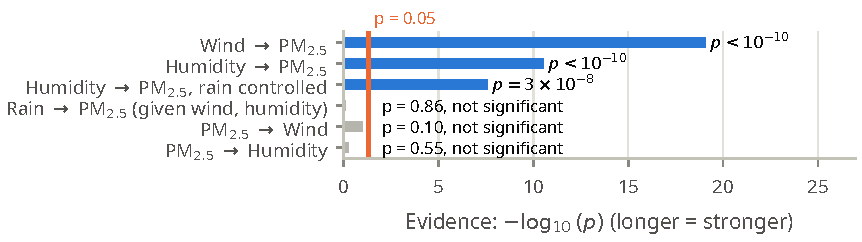
\includegraphics[width=0.9\linewidth]{granger_hac.pdf}\caption{HAC Wald tests (4 lags).}\end{figure}
\paragraph{Size and timing.} A one-SD wind shock (2.5 km/h) lowers \pmtwo{} by \irfWindA--\irfWindB\% the next day, a one-SD humidity shock (5.4\% RH) by \irfRhA--\irfRhB\%, fading within about a week; the range reflects the Cholesky ordering (weather first allows same-day effects). The generalised IRF, which does not depend on ordering, gives $-12.0\%$ and $-5.2\%$ on day 1, inside or at the edge of those ranges. Weather shocks explain \fevdA--\fevdB\% of the 14-day forecast-error variance of \pmtwo{} depending on the ordering.
\begin{figure}[H]\centering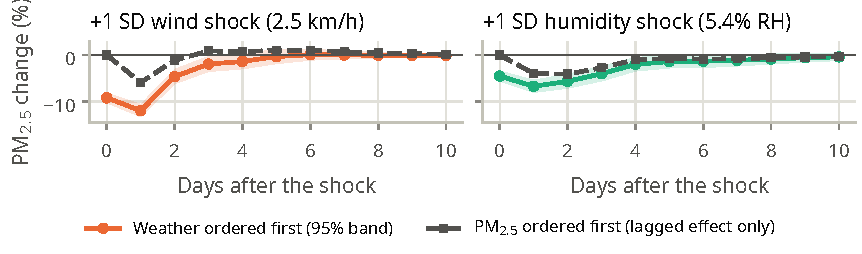
\includegraphics[width=0.95\linewidth]{irf_range.pdf}\caption{Impulse responses of \pmtwo{} to wind and humidity shocks under both orderings.}\end{figure}
\paragraph{Horizon.} At the weekly scale, last week's wind and humidity add nothing to last week's \pmtwo{} for predicting this week's ($\Delta R^2=0.005$, joint HAC Wald $p=0.51$). Weather is therefore a short-memory predictor, and the 52-week models use no weather.

\section{Forecasting (Q2)}\label{sec:fc}
\subsection{Models and evaluation design}
All models forecast weekly log \pmtwo{} with no weather inputs: seasonal naive; \textbf{climatology} (mean of each calendar week, benchmark); climatology + AR(1); \textbf{Fourier + ARMA} (dynamic harmonic regression: $K\le5$ yearly sine/cosine pairs, ARMA$(p,q)$ errors with $p\le2,q\le1$, and a level that is constant, linear or a random walk); SARIMA$(1,0,1)(0,1,1)_{52}$ and SARIMA$(1,0,1)(1,0,0)_{52}$ with a constant; Linear Regression on Fourier terms and a linear trend; and a small LSTM (16 units, recursive, seeded). For the Fourier model, $K$ and $(p,q)$ are chosen by AICc within each level type, and the level type by validation on the last training year; this procedure was declared the headline before any test year was inspected. Evaluation uses three expanding-window origins (end of 2016, 2017, 2018), each forecasting the next 52 weeks, refitting and reselecting every time. The 2017 fold (two training years) is a stress test; 2018 and 2019 are the main evidence. Paired error differences to climatology are summarised with a moving-block bootstrap (8-week blocks); a plain Diebold--Mariano test on 52 weeks of one forecast path is not valid and is not used here.
\begin{figure}[H]\centering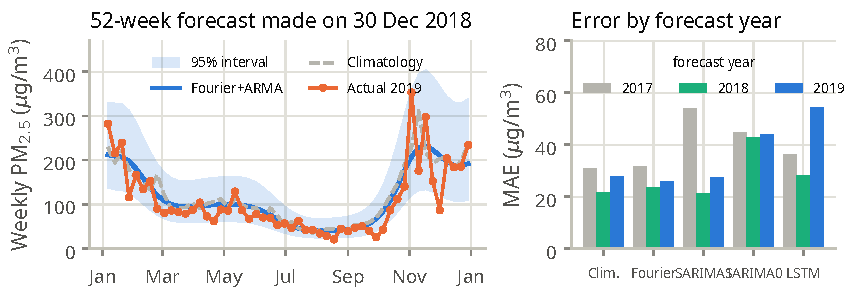
\includegraphics[width=0.95\linewidth]{fc_backtest.pdf}\caption{Left: the 2019 forecast of the selected model against climatology and the actual values. Right: MAE by forecast year.}\end{figure}
\subsection{Backtest results}
\begin{table}[H]\centering\footnotesize\begin{tabular}{lrrrrl}
\toprule
\textbf{Model} & \textbf{2017} & \textbf{2018} & \textbf{2019} & \textbf{Mean 18--19} & \textbf{vs climatology} \\
\midrule
Climatology (benchmark) & 31.0 & 21.8 & 27.8 & 24.8 & reference \\
Climatology + AR(1) & 30.7 & 21.7 & 27.3 & 24.5 & indistinguishable \\
Linear regression & 35.9 & 20.0 & 24.9 & 22.5 & indistinguishable \\
Fourier+ARMA (selected) & 31.5 & 23.4 & 25.7 & 24.6 & indistinguishable \\
SARIMA $D=1$ & 53.8 & 21.1 & 27.5 & 24.3 & indistinguishable \\
SARIMA $D=0$ (+constant) & 44.9 & 42.8 & 44.1 & 43.5 & worse \\
LSTM (small) & 36.3 & 28.3 & 54.3 & 41.3 & worse \\
Seasonal naive & 38.4 & 29.0 & 30.3 & 29.6 & worse \\
\bottomrule
\end{tabular}
\caption{52-week-ahead MAE (\ugm{}) by forecast year; last column: bootstrap verdict against climatology over 2018 and 2019.}\end{table}
In 2019 the selected Fourier+ARMA model has an MAE of \fcMaeSelNineteen{} against \fcMaeClimNineteen{} for climatology and \fcMaeSarimaNineteen{} for the seasonal-differenced SARIMA; the SARIMA is, however, at \fcMaeSarimaSeventeen{} in the 2017 fold, where it has only two seasons to learn from. Over 2018--2019 only the seasonal naive forecast, SARIMA with $D=0$ (\fcMaeSarimaZeroNineteen{} in 2019) and the LSTM (\fcMaeLstmNineteen{}) are clearly worse than climatology. The linear-trend Fourier variant is better on 2018--19 (the bootstrap interval excludes 0) but not over all three origins, and it was not the pre-declared choice, so we do not claim it. The honest summary: a year ahead the calendar carries almost all of the predictable signal, and with three origins the remaining models cannot be ranked.

\subsection{Diagnostics: errors in the earlier draft}
The draft's Ljung--Box test had $p\approx0$ at every lag. This was an artifact: a state-space SARIMA with $D=1$ initialises its first 52 seasonal states diffusely, so the first 52 in-sample residuals equal the level of the series (about 5 on the log scale). With them excluded (\texttt{loglikelihood\_burn}) the residuals are acceptable at lags 10 and 26 ($p=0.49,\,0.10$) but not at lag 52 ($p=0.016$). The seasonal MA coefficient is \fcMaCoef{} with a standard error far above 1: the parameter sits on the invertibility boundary and is not identified, the usual sign that the seasonal difference is unnecessary. The $D=0$ candidate in the draft had no constant, forcing the forecast toward $\log \text{PM}_{2.5}=0$; with a constant its validation MAE falls from 39.7 to 30.6 (but it remains the worst non-LSTM model overall). The selected Fourier+ARMA model still shows autocorrelation at lags 26 and 52 in the 2019 fold ($p=0.001$ and $0.009$) and ARCH-LM(4) is clean ($p=0.87$): there is more seasonal structure than a few harmonics capture, which we list as a limit.

\subsection{Prediction intervals}
Model-based 95\% intervals covered \fcCovRaw\% of the 2019 weeks; all misses were below the lower bound because 2019 was cleaner than 2015--18, so the problem is level bias as much as width. We rescale the predictive standard deviation by season (winter vs other months, shrunk toward the pooled value) using only the 2017 and 2018 errors, and re-centre only if the bias has the same sign and size $>0.5$ standard deviations in both calibration years; it did not (mean standardised errors $-0.66$ and $-0.45$), so only the scale is changed. On 2019 the calibrated coverage is \fcCovCal\%. The scale factors differ by fold (1.33/1.42 for 2019, 1.09/0.95 for the 2020 forecast), which shows the calibration is itself uncertain.

\subsection{One week ahead: does weather help?}
Each year 2018 and 2019 is forecast one week at a time with parameters fitted on earlier data. \emph{Lagged weather} (last week's wind and humidity anomalies) changes the error by \fcOneLagged\%, the \emph{last three days} of the previous week by \fcOneLastThree\%, and the \emph{same week's} weather (which is observed, not forecast, and so a hindsight upper bound) by \fcOneOracle\% (Harvey--Leybourne--Newbold $p=0.07$). Weather is explanatory over days, but a poor forecasting input.
\begin{figure}[H]\centering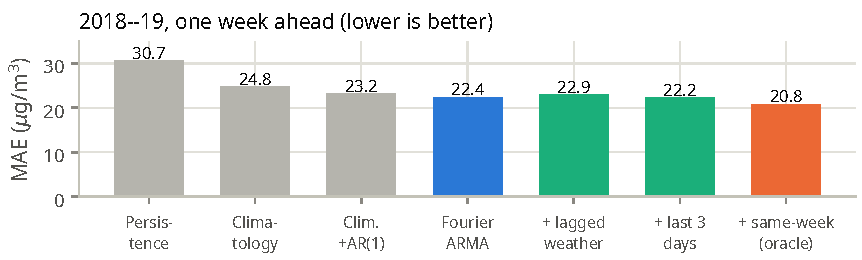
\includegraphics[width=0.7\linewidth]{fc_oneweek.pdf}\caption{One-week-ahead MAE, 2018--19.}\end{figure}

\subsection{The 2020 outlook and its validation}
The final model is fitted on 2015--2019 (selection again inside the window: linear level, $K=5$, AR(1) errors), 5{,}000 weekly paths are simulated, calibrated, converted to daily values by adding a within-week log offset resampled from the same calendar month of the training data, and classified into the CPCB \pmtwo{} bands. The same pipeline run for 2019 (data to 2018 only) places all \fcValInside{} monthly means inside the 95\% interval, but over-predicts the share of Poor-or-worse days (\fcValPoorPred\% vs \fcValPoorAct\% actual), which is the level bias again. These bands are \pmtwo{} sub-index bands, not the official AQI (the maximum over all pollutants).
\begin{figure}[H]\centering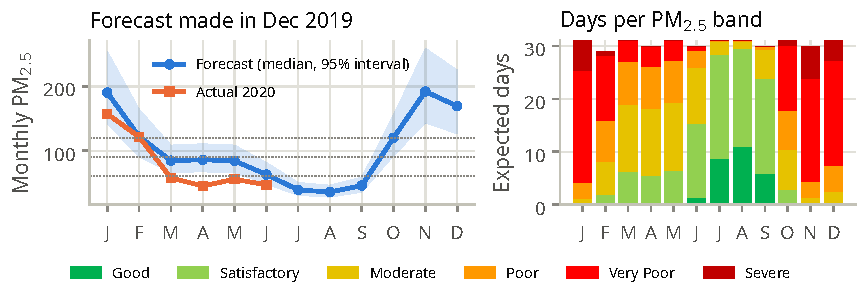
\includegraphics[width=0.95\linewidth]{fc_outlook.pdf}\caption{2020 outlook: monthly mean \pmtwo{} with 95\% interval and expected days per band.}\end{figure}
\begin{table}[H]\centering\scriptsize\begin{tabular}{|l|r|r|r|r|r|}
\hline
\textbf{Month} & \textbf{Median} & \textbf{95\% interval} & \textbf{P(mean$>$90)} & \textbf{Days Poor+} & \textbf{Actual} \\\hline
Jan & 190 & 143--254 & 100\% & 30 & 157 \\\hline
Feb & 121 & 90--164 & 98\% & 21 & 121 \\\hline
Mar & 85 & 66--109 & 32\% & 12 & 58 \\\hline
Apr & 86 & 67--112 & 35\% & 12 & 45 \\\hline
May & 85 & 67--109 & 33\% & 12 & 55 \\\hline
Jun & 63 & 48--81 & 0\% & 4 & 47 \\\hline
Jul & 39 & 30--50 & 0\% & 0 & -- \\\hline
Aug & 36 & 28--46 & 0\% & 0 & -- \\\hline
Sep & 45 & 35--59 & 0\% & 1 & -- \\\hline
Oct & 119 & 92--157 & 98\% & 21 & -- \\\hline
Nov & 192 & 143--258 & 100\% & 29 & -- \\\hline
Dec & 169 & 128--228 & 100\% & 29 & -- \\\hline
\end{tabular}
\caption{2020 outlook (\ugm{}); ``Days Poor+'' = expected days above 90 \ugm{}; Actual shown for full months only.}\end{table}
\subsection{Case study: the 2020 lockdown}
From 29 March to 31 May 2020 \pmtwo{} was about \fcLockPct\% below the no-lockdown forecast (95\% interval \fcLockLo--\fcLockHi\%). Using a version of the model that is given the actual wind and humidity of those weeks, the gap is \fcLockWxPct\%: most of the drop is not weather. This is descriptive; it depends on the forecast level for 2020 being right, which the interval calibration above shows is uncertain.
\begin{figure}[H]\centering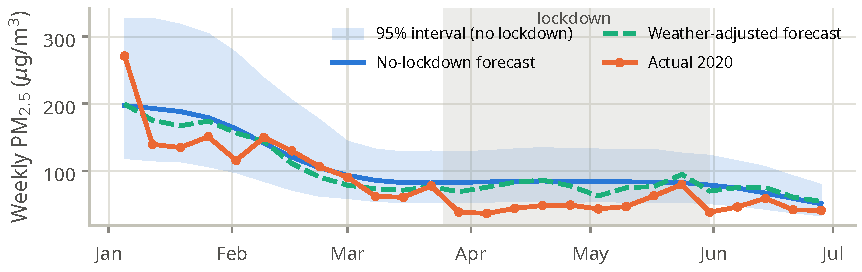
\includegraphics[width=0.85\linewidth]{fc_lockdown.pdf}\caption{Actual weekly \pmtwo{} in 2020 against the no-lockdown forecast and a weather-adjusted forecast.}\end{figure}

\section{Review of the project and what changed}\label{sec:review}
Three independent reviews proposed about 30 changes. We accepted the confirmed errors (diagnostic burn-in, missing constant, leakage in headline statistics, wording that over-stated causality or p-values, the PM$_{2.5}$-band versus AQI distinction, an invalid DM test) and rejected others after testing them (for example, the claim that re-anchoring the level gives 94\% coverage gives 90\% in the data; the shock-bin statistic has no Jensen bias; humidity's effect is not detectably monsoon-specific). The full log, with evidence for each claim, is \texttt{docs/REVIEW\_RESPONSES.md}.

\section{Limitations}
(i) Granger causality is predictive; boundary-layer height, stubble burning and fireworks are unmeasured, and ERA5 is a single grid cell. (ii) Three backtest origins give few independent tests; most model differences are not significant. (iii) A level bias remains: 2019 was cleaner than the training years, and the calibrated intervals depend on the fold. (iv) The Fourier model leaves some autocorrelation at lags 26 and 52. (v) One city; the data end in July 2020 and the monitoring network changed during the sample; the fixed-station check is small. (vi) The bands are \pmtwo{} sub-index bands, not the official AQI. (vii) The LSTM is deliberately small and is not tuned: it is a small-data negative result, not a statement about deep learning in general.

\section{Conclusion}
Delhi's \pmtwo{} is overwhelmingly a calendar phenomenon with a slowly falling level. Wind and humidity anomalies help for about a week, not for a year. For 52-week forecasts a smooth Fourier+ARMA model is as good as or marginally better than climatology and more robust than SARIMA, and its uncertainty can be calibrated; the forecast correctly isolates the 2020 lockdown. The most valuable parts of the work are the honest accounting of what is and is not significant and the correction of diagnostic errors that would have led to wrong model choices.

\section*{Reproducibility}
\texttt{pip install -r requirements.txt}; download the CPCB files (Section~2) and run notebooks 01--04; then \texttt{python slides/beamer/make\_figures.py}, \texttt{python slides/beamer/verify\_numbers.py} (65 independent checks of every number on the slides) and build \texttt{slides/beamer/main.tex} and this report with \texttt{tectonic}. Code: \texttt{src/} (data, tsa, forecast, aqi, plots).
\end{document}
